\subsubsection{Soft USART driver in detail}
\label{sec:bus:design:layer1:interface:swuart}

The software USART driver is designed in such a way as it takes only data via methods and returns data only via callback routines (which can be seen as events).\\

The methods provided by the driver are

\begin{enumerate}
 \item \textbf{initialize: } initializes the sw usart driver and configures it with certain parameters such as the baud rate and the callback methods triggered on event occurences.
 \item \textbf{writeByte: } takes a byte of data and transmitts it.
\end{enumerate}

and the events provided by the driver are

\begin{enumerate}
 \item \textbf{startBitDetectedCallback}
 \item \textbf{byteTransmittedCallback}
 \item \textbf{byteCorruptedCallback}
\end{enumerate}

\begin{figure}[h]
\centering
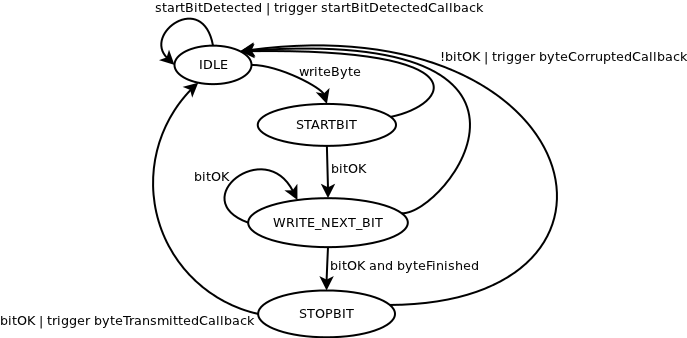
\includegraphics[width=0.8\textwidth]{../images/swuart_statemachine.png}
\caption{Soft USART Driver State Machine.}
\label{fig:bus:design:layer1:interface:swuart}
\end{figure}

The workflow of the drivers statemachine depicted in figure \ref{fig:bus:design:layer1:interface:swuart} starts in the state \textit{IDLE}.\\

When data is pushed into the driver via the \textit{writeByte} method the transmission via the usart simulation is initiated and the statemachine changes to state \textit{STARTBIT} in which the startbit of the USART Message is written to the bus.\\

If the bit represented on the bus equals the startbit written the driver moves to state \textit{WRITE\_NEXT\_BIT} in which the bits of the byte to be written are written to the bus.\\

After all eight bits to be transmitted could be bitwise read in correctly again the driver sends the stopbit in the state \textit{STOPBIT} and triggers the \textit{byteTransmittedCallback} event on success.\\

Otherwise if any bit written to the bus could not read back correctly the statemachine triggers the event \textit{byteCorruptedCallback} and goes to state \textit{IDLE}.\\

A very important event for our protocol with respect to performance of the higher layers is given by \textit{startBitDetectedCallback} which is triggered whenever a start of a message is detected in the \textit{IDLE} state.\\